\begin{frame}
 \frametitle{Demo 10 $\vert$ \bfseries Finite Element Method}
 \framesubtitle{\bfseries Plate with circular hole under simple tension}
%  \hspace*{-1em}
 
  \begin{tikzpicture}  
   \draw[decoration={random steps, amplitude=1pt, segment length=1mm}, decorate] (-2, -2) -- ++(4, 0) -- ++(0, 4) -- ++(-4, 0) -- ++(0, -4);
   \begin{scope}[rotate=45, scale=1.3]
%      \draw[thick] (0, 0) circle [x radius=1cm, y radius=0.5cm];
     \draw[thick] (0, 0) circle [x radius=0.5cm, y radius=0.5cm];
%      \draw[dashed] (0, 0) -- node[above,yshift=0mm]{\(a\)} (1, 0);
%      \draw[dashed] (0, 0) -- node[below left, xshift=1mm, yshift=1mm]{\(b\)} (0, 0.5);
   \end{scope}
%    \draw[-latex] (0, 0) -- +(1.4, 0) node[above]{\(x\)}; 
%    \draw[-latex] (0, 0) -- +(0, 1.4) node[above, yshift=-1mm]{\(y\)}; 
%    \draw[latex-latex,red] (0.7, 0) arc (0:45:0.7) node[below, xshift=-2pt, yshift=-1pt]{\(\beta\)};
   \begin{scope}[yscale=0.9]
    \foreach \x in {-2, -1, 0, 1, 2} {
     \draw[-latex, ultra thick, xshift=1mm] (2, \x) -- +(0.7, 0);
     \draw[-latex, ultra thick, xshift=-1mm] (-2, \x) -- +(-0.7, 0);
    }
   \end{scope}
  \draw (2, 2) node[above right, xshift=2mm]{\(\v t^p\)};
%   \draw (-2, -2) node[above right]{\(S\)};

  \begin{scope}[xshift=5.6cm]
    \draw (0, 0) node{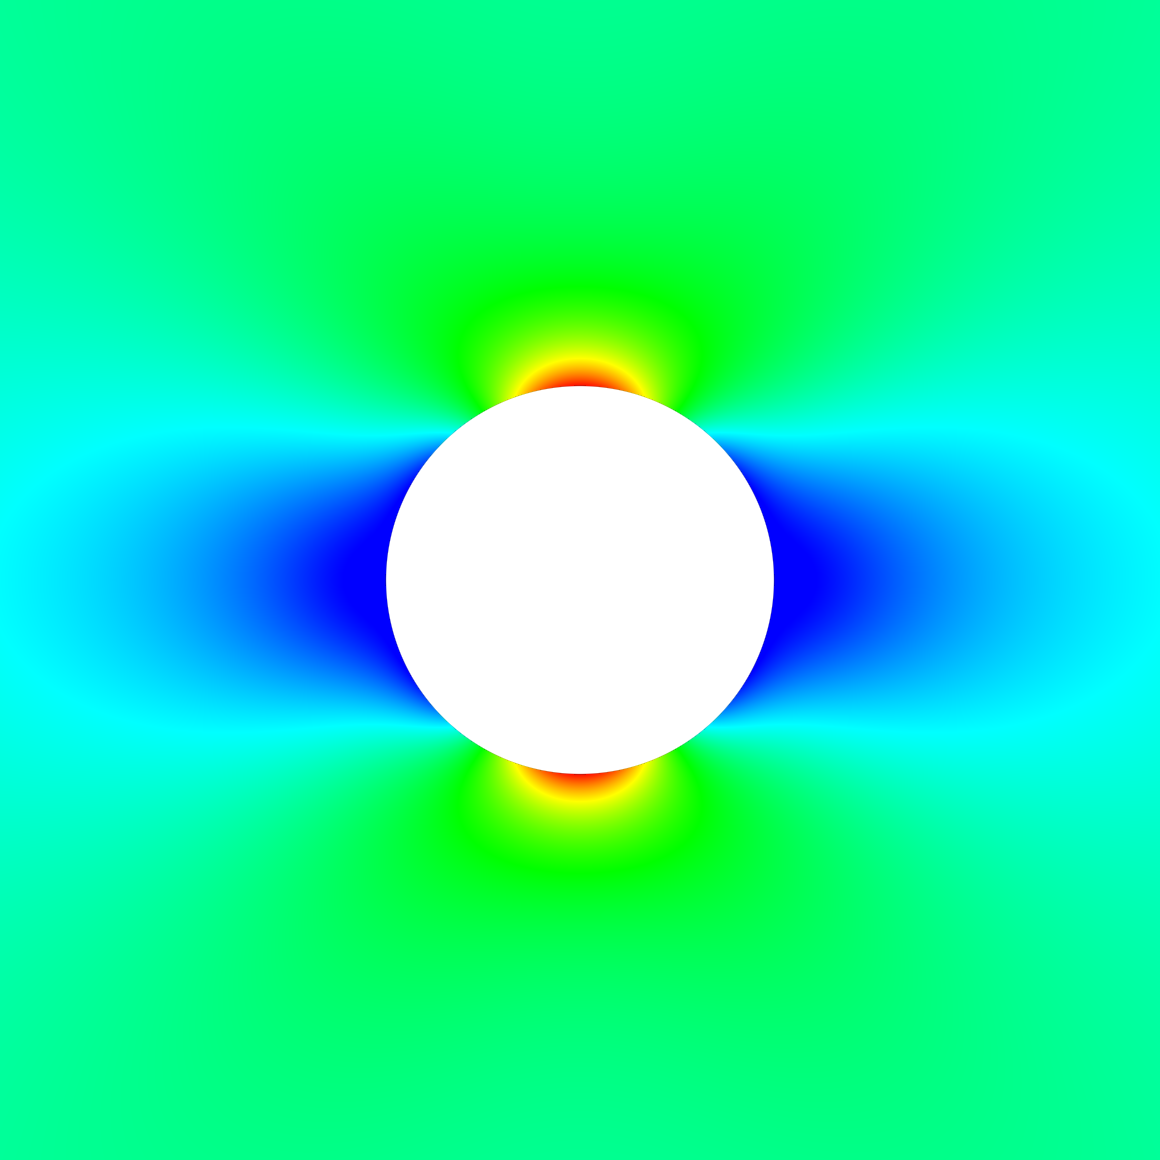
\includegraphics[height=4cm]{../10-plate/plate_full}};
%    \draw (-2, -2) rectangle (2, 2);
%    \begin{axis}[verticalbar,point meta min=0,point meta max=3,colorbar/.append style={ytick={0,1,2,3}}] \addplot [draw=none] coordinates {(0,0)}; \end{axis}
%    \draw (0, 0) node[above right, xshift=2.1cm,yshift=2cm]{\(\sigmaxx\)};
   \end{scope}

%    \node at (-3, -2.1) {a)};
%    \node at (3.3, -2.1) {b)};
  \end{tikzpicture}

%   \begin{tikzpicture}  
%   \begin{scope}[xshift=8.3cm,yshift=1.1cm,scale=1.1]
%    \begin{axis}[stressbar,point meta min=0,point meta max=3.4,title={$\sigma_{11}$}]
%    \addplot [draw=none] coordinates {(0,0)}; \end{axis}
%   \end{scope}
%  \end{tikzpicture}

 \vspace*{2ex}
  \centering
  Analytical solution available, visit \\[1ex]
  \textit{www.ltm.fau.de/plate} \\[1ex]
  for visualization and further references.

\end{frame}

\begin{frame}
 \frametitle{Demo 10 $\vert$ \bfseries Finite Element Method}
 \framesubtitle{\bfseries Plate with circular hole under simple tension}
%  \hspace*{-1em}
 \begin{tikzpicture}[]
  \node at(0, 2.6) {Mesh};
  \node at(5, 2.6) {Solution};
  \only<1>{
    \node at(0,0) {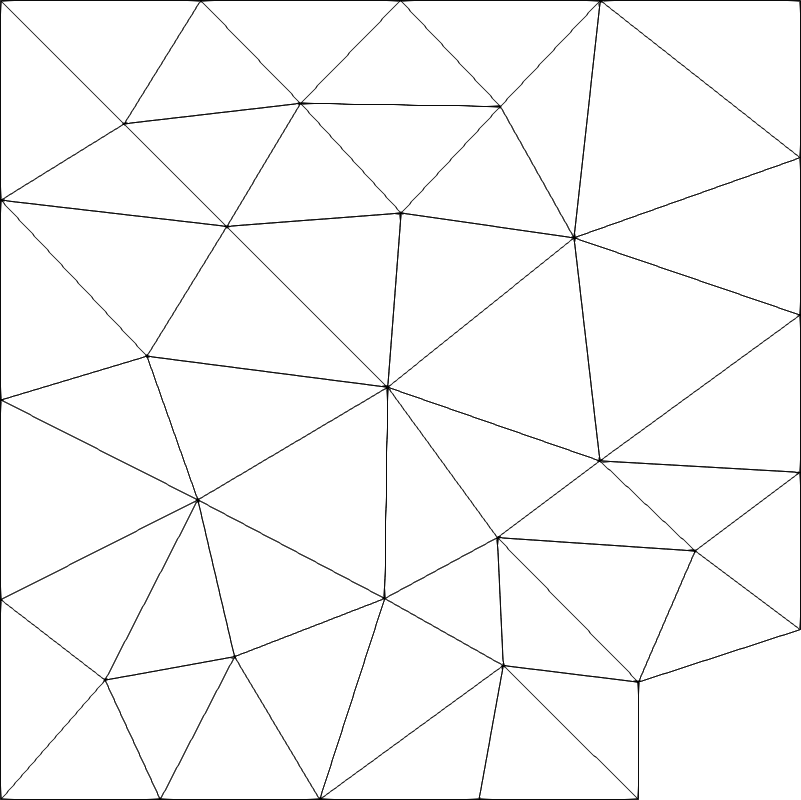
\includegraphics[width=4.4cm]{../10-plate/mesh_0.png}};
    \node at(5,0) {
\includegraphics[width=4.4cm]{../10-plate/solution_0.png}};
    \node at(-2.3, -3)[right] {Number of elements: $48$};
  }
  \only<2>{
    \node at(0,0) {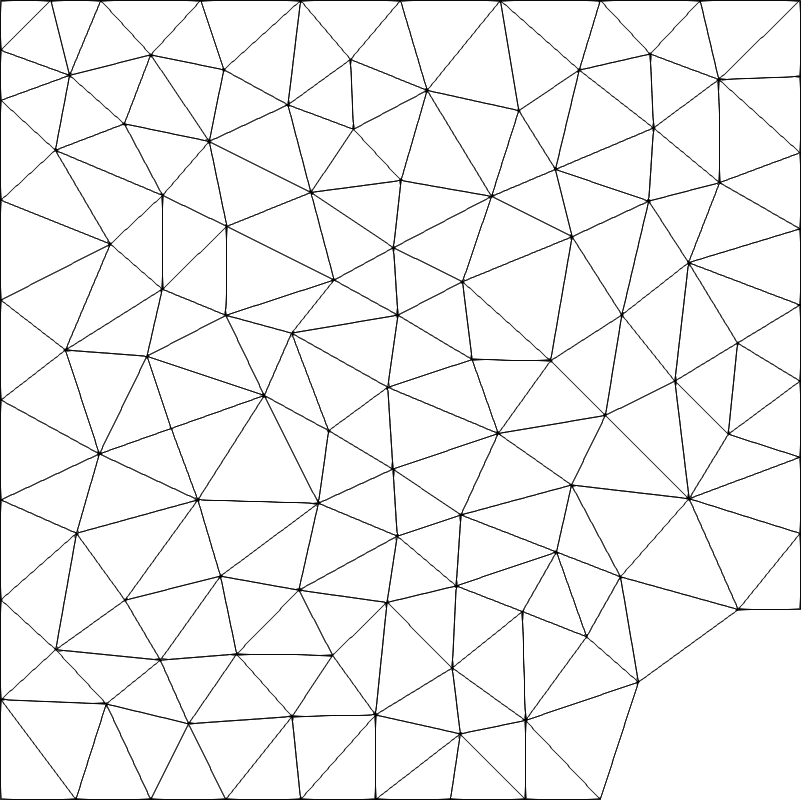
\includegraphics[width=4.4cm]{../10-plate/mesh_1.png}};
    \node at(5,0) {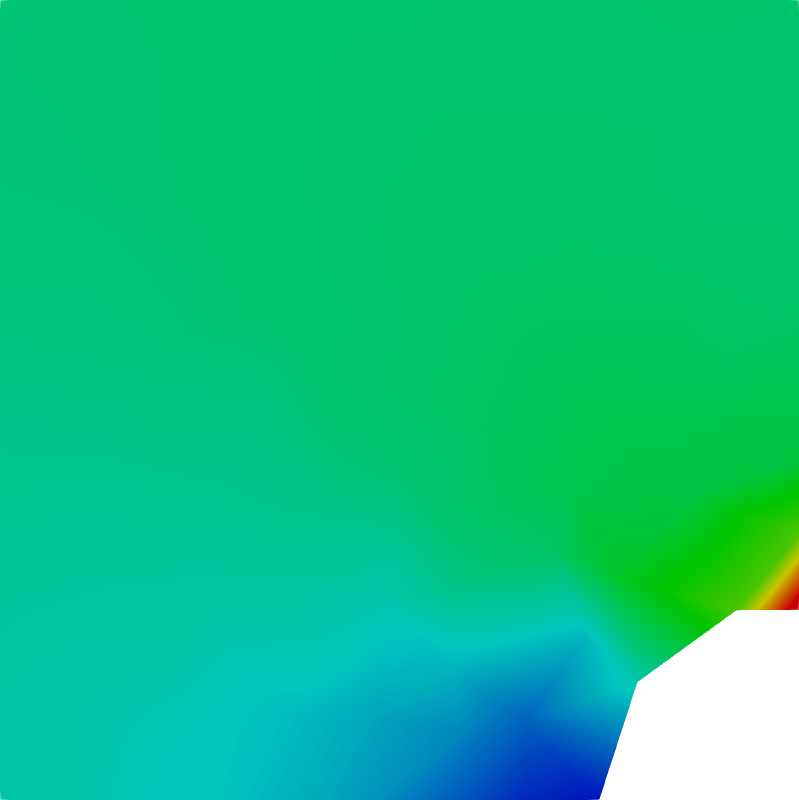
\includegraphics[width=4.4cm]{../10-plate/solution_1.png}};
    \node at(-2.3, -3)[right] {Number of elements: $187$};
  }
  \only<3>{
    \node at(0,0) {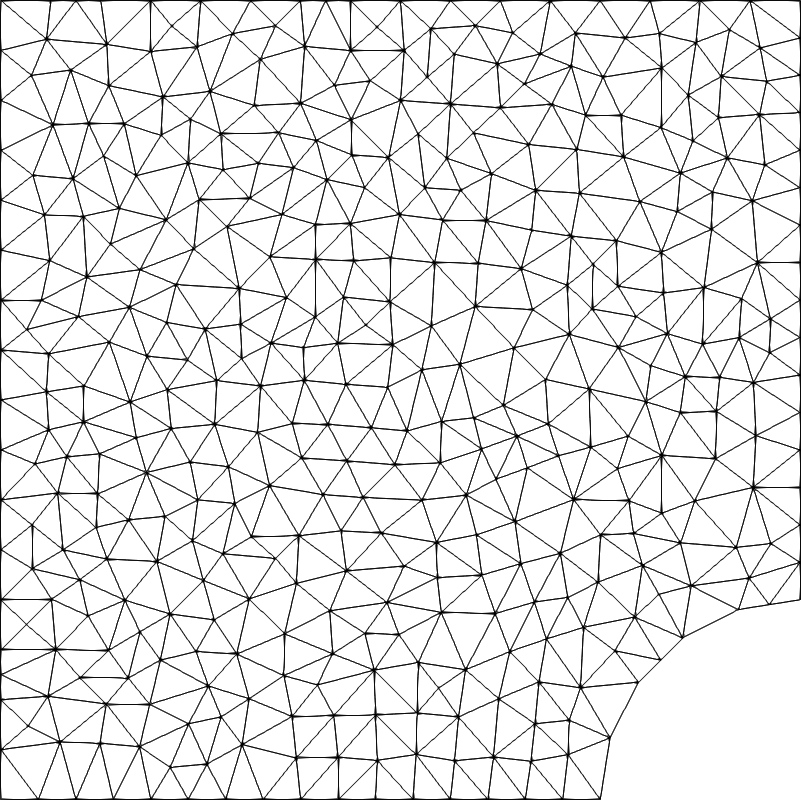
\includegraphics[width=4.4cm]{../10-plate/mesh_2.png}};
    \node at(5,0) {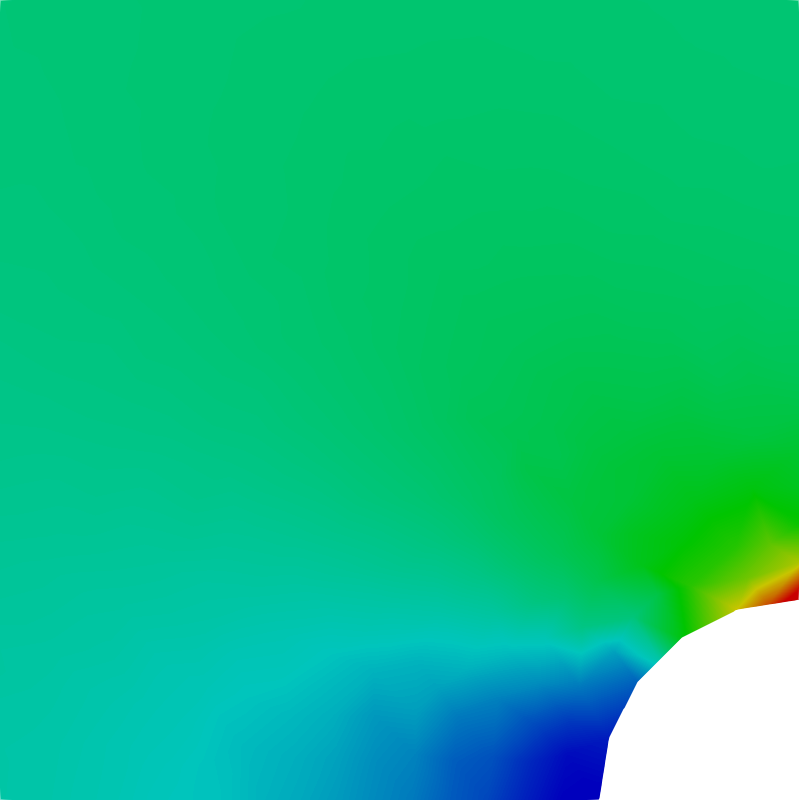
\includegraphics[width=4.4cm]{../10-plate/solution_2.png}};
    \node at(-2.3, -3)[right] {Number of elements: $746$};  
  }
  \only<4>{
    \node at(0,0) {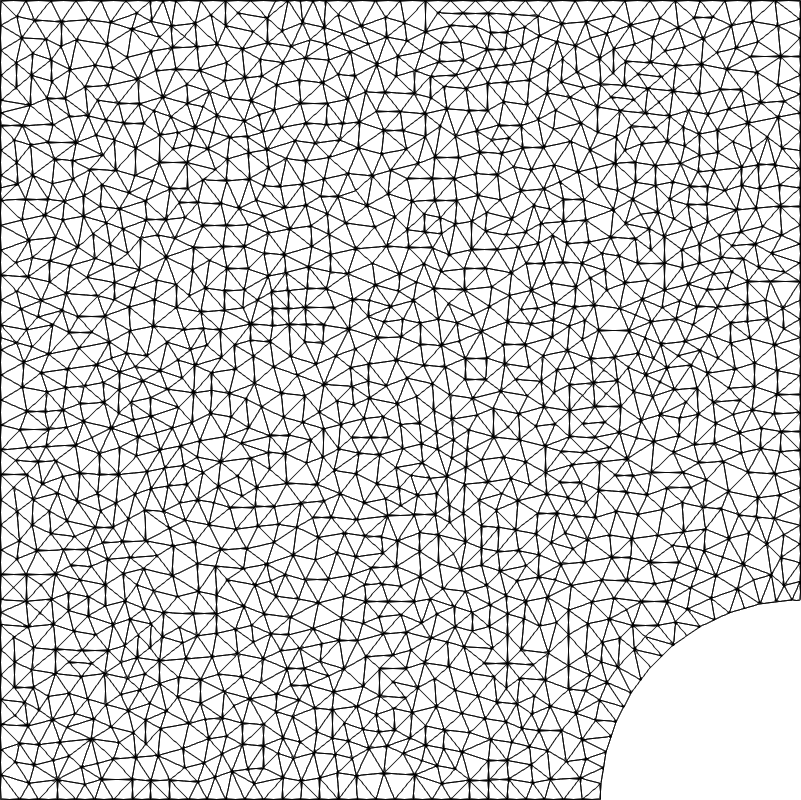
\includegraphics[width=4.4cm]{../10-plate/mesh_3.png}};
    \node at(5,0) {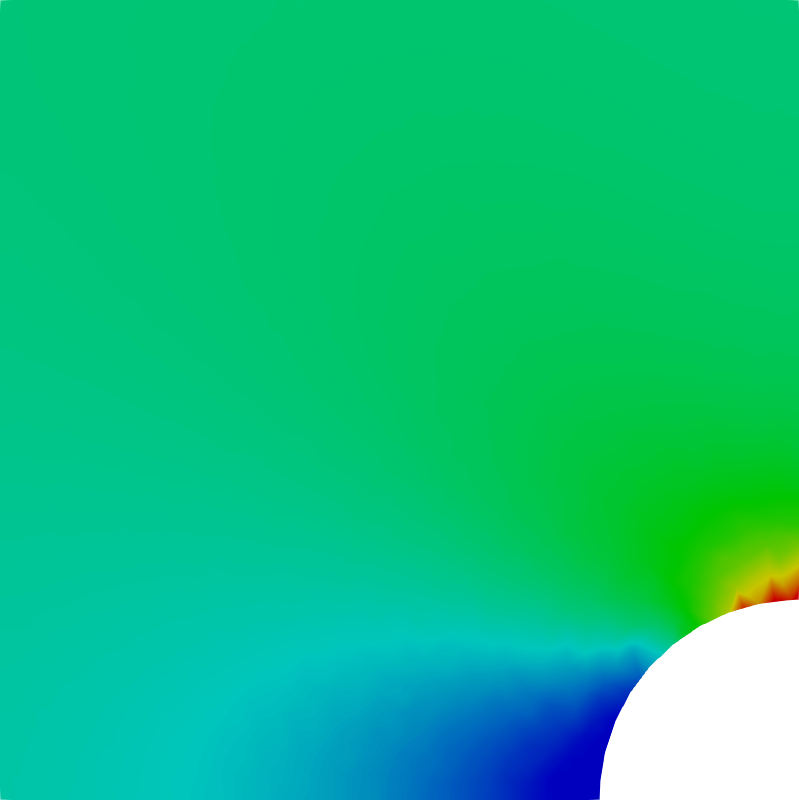
\includegraphics[width=4.4cm]{../10-plate/solution_3.png}};
    \node at(-2.3, -3)[right] {Number of elements: $3013$};  
  }
  \only<5>{
    \node at(0,0) {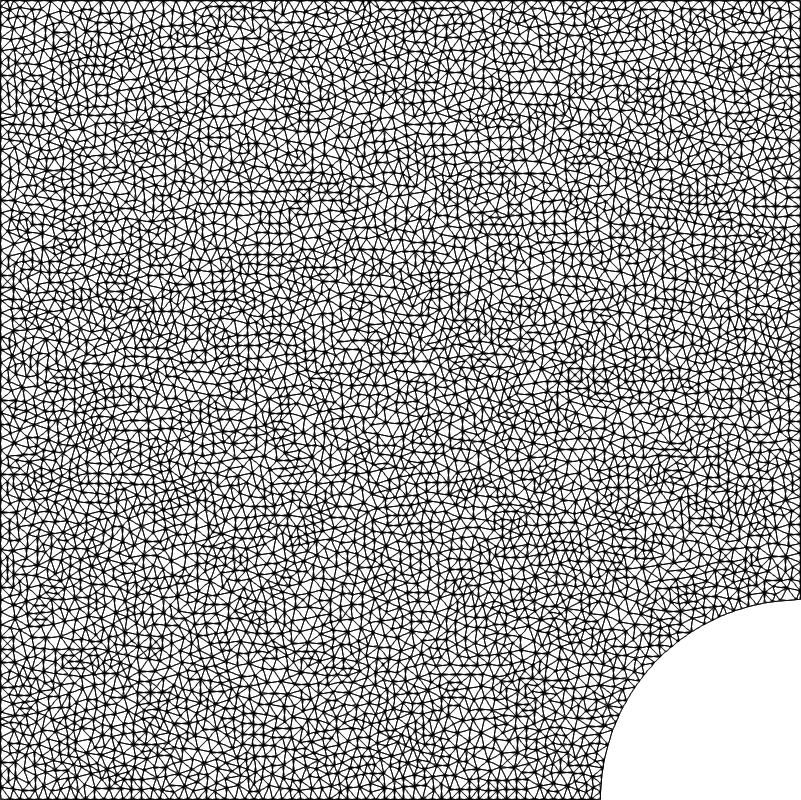
\includegraphics[width=4.4cm]{../10-plate/mesh_4.png}};
    \node at(5,0) {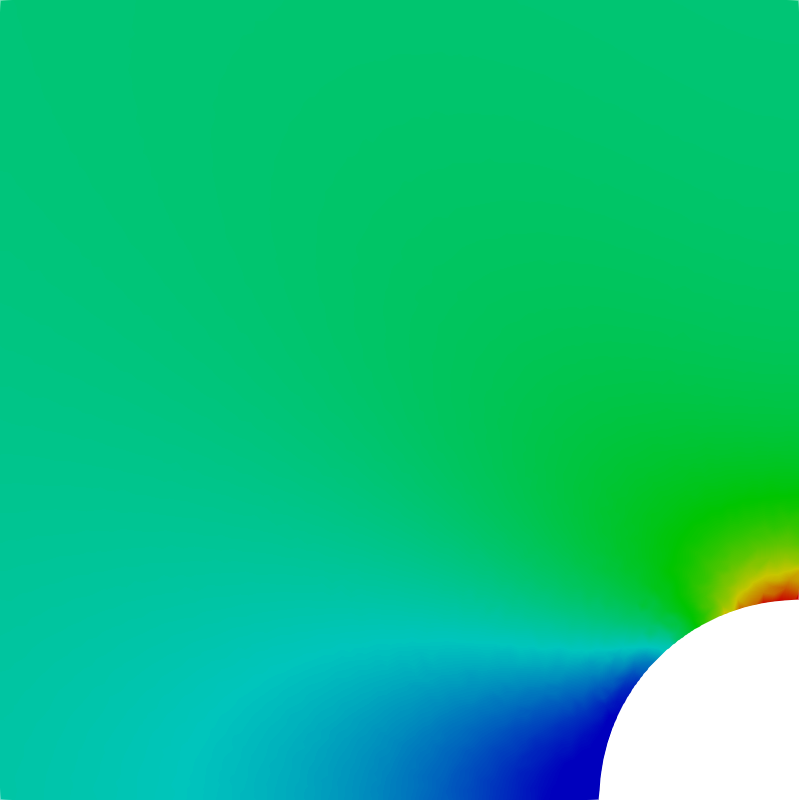
\includegraphics[width=4.4cm]{../10-plate/solution_4.png}};
    \node at(-2.3, -3)[right] {Number of elements: $11989$};  
  }
  \only<6>{
    \node at(0,0) {
\includegraphics[width=4.4cm]{../10-plate/mesh_5.png}};
    \node at(5,0) {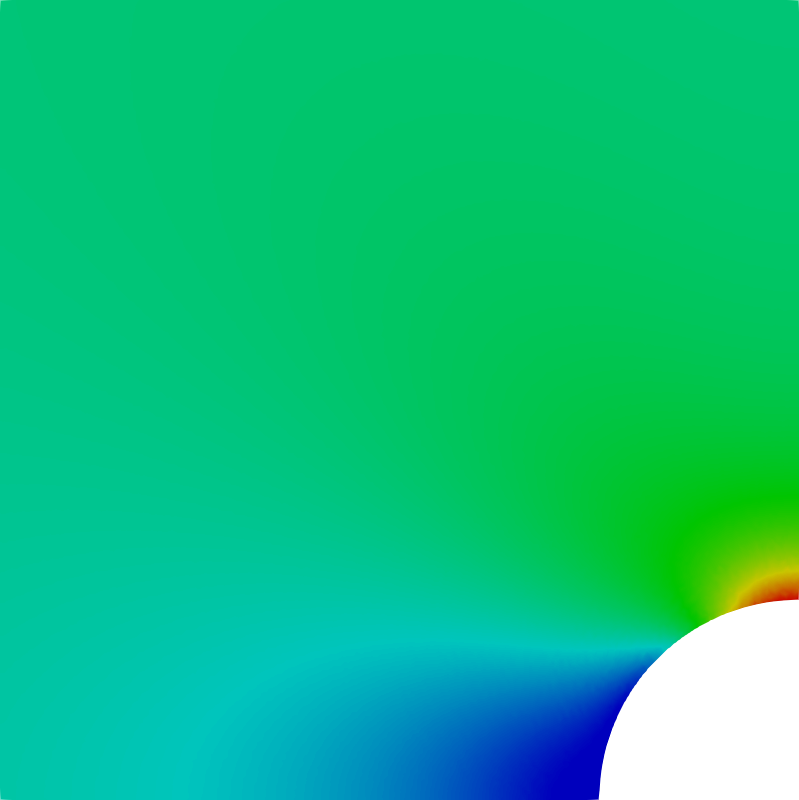
\includegraphics[width=4.4cm]{../10-plate/solution_5.png}};
    \node at(-2.3, -3)[right] {Number of elements: $48425$};
  }  
  \only<7>{
    \node at(0,0) {
\includegraphics[width=4.4cm]{../10-plate/mesh_6.png}};
    \node at(5,0) {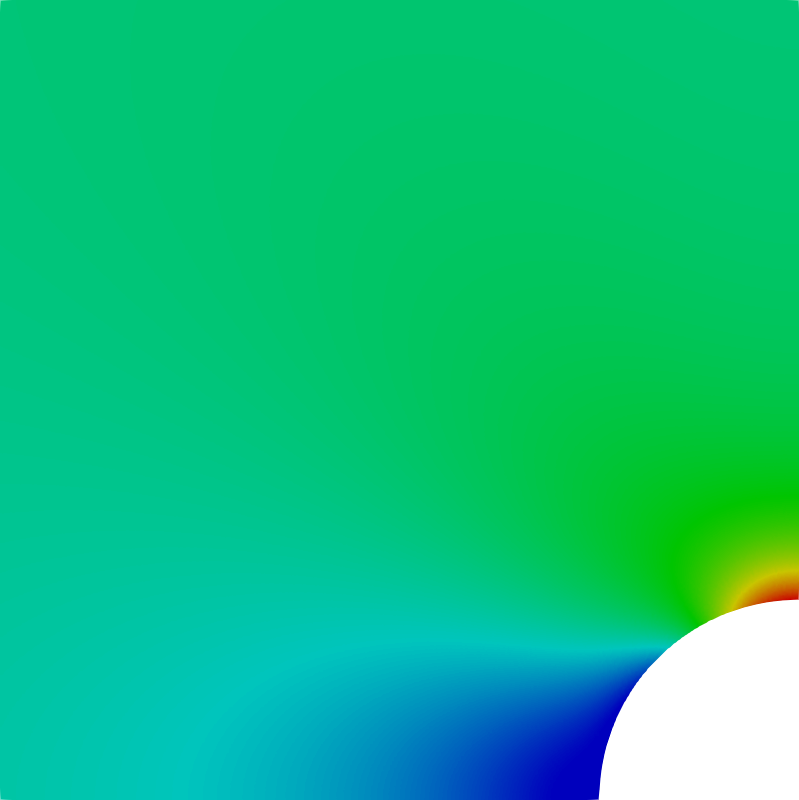
\includegraphics[width=4.4cm]{../10-plate/solution_6.png}};
    \node at(-2.3, -3)[right] {Number of elements: $193349$};  
  }
  \only<8>{
    \node at(0,0) {
\includegraphics[width=4.4cm]{../10-plate/mesh_7.png}};
    \node at(5,0) {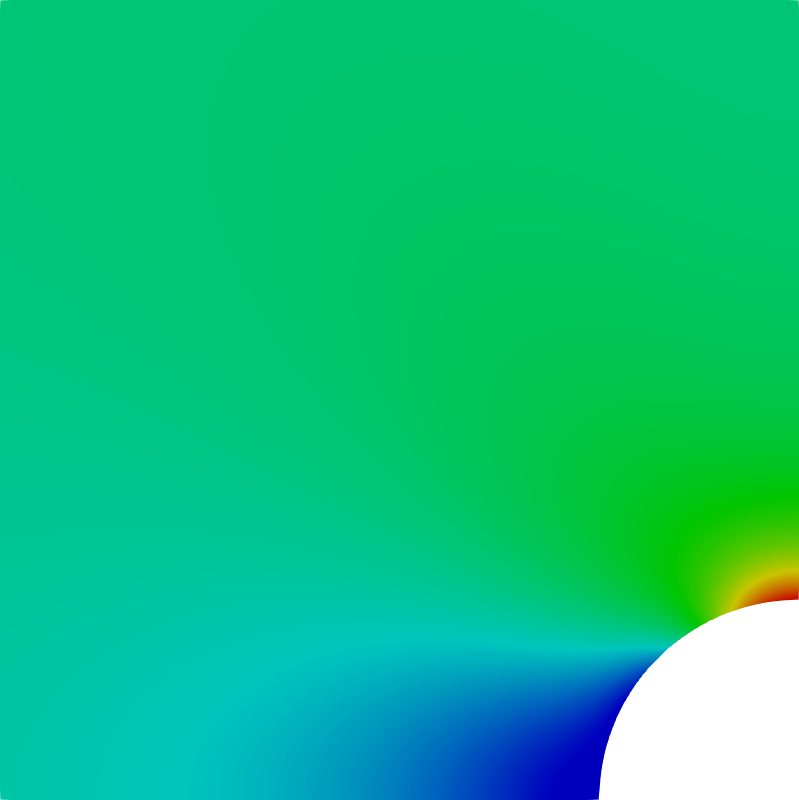
\includegraphics[width=4.4cm]{../10-plate/solution_7.png}};
    \node at(-2.3, -3)[right] {Number of elements: $772466$};
  }

  \begin{scope}[xshift=8.3cm,yshift=1.1cm,scale=1.1]
   \begin{axis}[stressbar,point meta min=0,point meta max=3,title={$\sigma_{11}$}]
   \addplot [draw=none] coordinates {(0,0)}; \end{axis}
  \end{scope}   
 \end{tikzpicture}
\end{frame}
 

\begin{frame}
 \frametitle{Demo 10 $\vert$ \bfseries Finite Element Method}
 \framesubtitle{\bfseries Plate with circular hole under simple tension}
 \hspace*{-1em}
 \begin{tikzpicture}[scale=0.63]
  \begin{loglogaxis}[title={Error}, legend pos=south west, xlabel={$h_{\mathrm{max}}$}, ylabel={$\Vert \v \sigma^h - \v \sigma \Vert_{L^2(\mathcal{B})}$}, x dir=reverse]
   \addplot[blue,mark=*] table[x={hmax},y={error}] {../10-plate/history1.dat};
   \addplot[red,mark=*] table[x={hmax},y={error}] {../10-plate/history2.dat};
%    \addplot[gray,mark=o] table[x={hmax},y={error}] {../10-plate/history3.dat};
   \legend{$p=1$,$p=2$,$p=3$,$p=4$}
  \end{loglogaxis}
 \end{tikzpicture}
 \hfill
 \begin{tikzpicture}[scale=0.63]
  \begin{loglogaxis}[title={Computing time}, legend pos=north west, xlabel={$h_{\mathrm{max}}$}, ylabel={wall clock in sec.}, x dir=reverse]
   \addplot[blue,mark=*] table[x={hmax},y={clock_solve}] {../10-plate/history1.dat};
   \addplot[red,mark=*] table[x={hmax},y={clock_solve}] {../10-plate/history2.dat};
%    \addplot[gray,mark=o] table[x={hmax},y={clock_solve}] {../10-plate/history3.dat};
   \legend{$p=1$,$p=2$,$p=3$,$p=4$}
  \end{loglogaxis}
 \end{tikzpicture}
\end{frame}
 